\documentclass[11pt, letterpaper]{article}
\usepackage[utf8]{inputenc}

\makeatletter
\newcommand{\@BIBLABEL}{\@emptybiblabel}
\newcommand{\@emptybiblabel}[1]{}
\newcommand*{\permcomb}[4][0mu]{{{}^{#3}\mkern#1#2_{#4}}}
\newcommand{\perm}[1][-3mu]{\permcomb[#1]{P}}
\makeatother
\usepackage[hidelinks]{hyperref}
\usepackage{comment}
\usepackage{enumitem}
\usepackage{fullpage}
\usepackage[english]{babel}
\usepackage{graphicx}
\usepackage[colorinlistoftodos]{todonotes}
\usepackage[linesnumbered]{algorithm2e}
\usepackage{tabularx}
\usepackage{url}
\usepackage{hyperref}
\hypersetup{colorlinks=true}
\usepackage[margin=0.7in]{geometry}    % For reducing margin
\usepackage[english]{babel}
\usepackage{mathtools}
\usepackage{booktabs}
\usepackage{physics}
\usepackage{amsmath,amssymb,amsthm}
\usepackage{fullpage}
\usepackage{enumitem}
\usepackage{tcolorbox}
\usepackage{comment}
\usepackage{framed}

\newcommand{\wx}[1]{\textcolor{magenta}{\bf\small [#1 --WX]}}

\begin{document}

\title{CS 4650: Natural Language Processing (Spring 2023) \\ Problem Set 2}
\author{Instructor: Wei Xu \\ TAs: Rahul Katre, Marcus Ma, Mounica Maddela, Ben Podrazhansky
\\Piazza: \url{https://piazza.com/gatech/spring2023/cs4650}
\\Gradescope: \url{https://www.gradescope.com/courses/481426}}
\date{Due: Thursday, March 16, 11:59 PM ET}
\maketitle

\section{Understanding Word2Vec}
Given a sequence of words $w_{1}, \ldots, w_{T}$ and context size $c$, the training objective of skip-gram is:
$$
\mathcal{L}=-\frac{1}{T} \sum_{t=1}^{T} \sum_{-c \leq j \leq c, j \neq 0} \log P\left(w_{t+j} \mid w_{t}\right)
$$
where $P\left(w_{o} \mid w_{t}\right)$ is defined as:
$$
P\left(w_{o} \mid w_{t}\right)=\frac{\exp \left(\mathbf{u}_{w_{t}}^{\top} \mathbf{v}_{w_{o}}\right)}{\sum_{k \in V} \exp \left(\mathbf{u}_{w_{t}}^{\top} \mathbf{v}_{k}\right)}
$$
where $\mathbf{u}_{k}$ represents the ``target" vector and $\mathbf{v}_{k}$ represents the``context" vector, for every $k \in V$.\\
\begin{enumerate}[label=(\alph*)]
\item (\textbf{3 pts}) Derive the following gradient (probability w.r.t context vector):
$$
-\frac{\partial \log P\left(w_{o} \mid w_{t}\right)}{\partial \mathbf{v}_{w_{o}}}
$$

\item (\textbf{2 pts}) Imagine that we train the model on a large corpus (e.g. English Wikipedia). Describe the effects of context size $c$ to the resulting word vectors $\mathbf{u}_{w}$, i.e. what if we use context size $c=1,5$, or $100 ?$\\\\

\end{enumerate}

\newpage

\section{Hidden Markov Models and the Viterbi Algorithm}
    We have a toy language with 2 words - “cool” and “shade”. We want to tag the parts of speech in a test corpus in this toy language. There are only 2 parts of speech — NN (noun) and VB (verb) in this language. We have a corpus of text in which we the following distribution of the 2 words:
    
    \begin{table}[h!]
    \centering
    \small
    \begin{tabular}{|l | c | c |}
    \hline & NN & VB\\
    \hline
    cool & 3 & 6 \\
    shade & 7 & 4\\
    \hline
    \end{tabular}
    \end{table}
    Assume that we have an HMM model with the following transition probabilities (* is a special start of the sentence symbol).
    
    \begin{figure}[h]
    \centering
    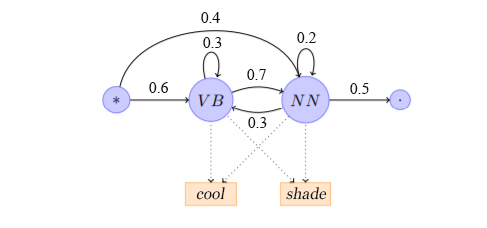
\includegraphics{images/HMM.jpg}
    \caption{HMM model for POS tagging in our toy language.}
    \end{figure}

\begin{enumerate}[label=(\alph*)]
\item (\textbf{2 pts}) Compute the emission probabilities for each word given each POS tag.\\

\item (\textbf{3 pts}) Draw the Viterbi trellis for the sequence “cool shade.”. Highlight the most likely sequence. \href{https://web.stanford.edu/~jurafsky/slp3/A.pdf#page=8}{\color{blue}{Here}} is an  example of Viterbi trellis.

\end{enumerate}

\newpage

\section{LSTMs}


The update equations for a LSTM at timestep $i$ are given in the following equations. Eisenstein Chapter 6.3 may be useful in answering this question. 
% \begin{figure}[h!]
%     \centering
%     \includegraphics[width=0.8\textwidth]{images/midterm_images/lstm.png}
%     \caption{LSTM update equations (Eisenstein Ch. 6.33).}
%     \label{fig:lstm}
% \end{figure}

\begin{align*} 
    \mathbf{f_i} &= \sigma(\mathbf{W}^{(f)} \mathbf{h_{i-1}} + \mathbf{U}^{(f)} \mathbf{x_{i}}    + \mathbf{B}^{(f)} ) \qquad   &\text{Forget gate} \\
    \mathbf{i_i} &= \sigma(\mathbf{W}^{(i)} \mathbf{h_{i-1}} + \mathbf{U}^{(i)} \mathbf{x_{i}}   + \mathbf{B}^{(i)} ) \qquad  &\text{Input gate} \\
    \mathbf{g_i} &= tanh(\mathbf{W}^{(g)} \mathbf{h_{i-1}} + \mathbf{U}^{(g)} \mathbf{x_{i}} )  \qquad   &\text{Update candidate}\\
    \mathbf{c_i} &= \mathbf{f_i} \odot \mathbf{c}_{i-1}  + \mathbf{i_i} \odot \mathbf{g_i}  \qquad   &\text{Memory cell update}\\
    \mathbf{o_i} &= \sigma(\mathbf{W}^{(o)} \mathbf{h_{i-1}} + \mathbf{U}^{(o)} \mathbf{x_{i}}   + \mathbf{B}^{(o)} ) \qquad   &\text{Output gate}\\
    \mathbf{h_i} &= \mathbf{o_i} \cdot \text{tanh}(\mathbf{c_i})  \qquad   &\text{Output} 
\end{align*} 



\begin{enumerate}[label=(\alph*)]

\begin{table}[h]
    \centering
    \begin{tabular}{|cc|}
    \toprule
    \textbf{Weight} & \textbf{Value} \\
    \midrule
    $\mathbf{W}^{(f)}$ & $[1,-2,-3]$ \\
    $\mathbf{U}^{(f)}$ & $[0,-1,-2]$ \\
    $\mathbf{B}^{(f)}$ & $0$ \\
    $\mathbf{W}^{(i)}$ & $[0,0,1]$\\
    $\mathbf{U}^{(i)}$ & $[-1,-2,-2]$\\
    $\mathbf{B}^{(i)}$ & $1$ \\
    $\mathbf{W}^{(g)}$ & $\begin{bmatrix}
    0 & 1 & -3\\
    -3 & 1 & 0\\
    -2 & -1 & -3
        \end{bmatrix}$ \\
    $\mathbf{U}^{(g)}$ & $\begin{bmatrix}
    1 & 0 & 0 \\
    -2 & -3 & 0\\
    1 & -1 & -2 \end{bmatrix}$ \\
    $\mathbf{W}^{(o)}$ & $[1,0,1]$\\
    $\mathbf{U}^{(o)}$ & $[-1,0,1]$\\
    $\mathbf{B}^{(o)}$ & $-1$ \\
    \bottomrule
    \end{tabular}
    \caption{Weights for LSTM.}
    \label{tab:lstm_weights}
\end{table}

\newpage

\item (\textbf{1 pt}) In \autoref{tab:lstm_weights} we provide weight values and in \autoref{tab:lstm_intvars} timestep inputs. We'll now compute the value of $\boldsymbol{h}_{i}$ using \autoref{tab:lstm_weights} and \autoref{tab:lstm_intvars}: 

\begin{table}[h!]
    \centering
    \begin{tabular}{|cc|}
    \toprule
    \textbf{Vector} & \textbf{Value} \\
    \midrule
    $\boldsymbol{h}_{i-1}$ & $[3,1,-1]^T$ \\
    $\boldsymbol{c}_{i-1}$ & $[1,0,-4]^T$ \\
    $\boldsymbol{x}_{i}$ & $[-3,-2,-1]^T$ \\
    \bottomrule
    \end{tabular}
    \caption{Input/intermediate variables for LSTM.}
    \label{tab:lstm_intvars}
\end{table}


$\boldsymbol{f}_{i} = \sigma(4 + 4 + 0) = 1.0$ \\
\indent $\boldsymbol{i}_{i} = \sigma(-1 + 9 + 1) = 1.0$ \\
\indent $\boldsymbol{g}_{i} = \text{tanh}([4, -8, -4]^T + [-3, 12, 1]^T) = \text{tanh}([1,4,-3]^T) = [0.76, 1.0, -1.0]^T$\\
\indent $\boldsymbol{c}_{i} = 1.0 \odot [1,0,-4]^T + 1.0 \odot [0.76, 1.0, -1.0]^T = [1.76, 1.0, -5.0]^T $ \\
\indent $\boldsymbol{o}_{i} = \sigma(2 + 2 - 1) = 1.0$\\
\indent $\boldsymbol{h}_{i} = 1.0 \odot \text{tanh}([1.76, 1.0, -5.0]^T) = \mathbf{[0.94, 0.76, -1.0]^T}$\\

\textbf{Note that this is just a toy example of an LSTM layer where the gate values are scalars. In a real LSTM such as the one in PyTorch, the gate values will be vectors with some hidden layer dimensionality.}


The gates of this LSTM do not restrict the flow of any information. To effectively turn this LSTM into an Elman RNN at the current timestep, i.e., include \textbf{only} information from the current input and prior hidden state and \textbf{no} information from the prior memory cell in $\boldsymbol{h}_{i}$, describe the values that you would need to set the gates $\boldsymbol{f}_{i}, \boldsymbol{i}_{i}$ and $\boldsymbol{o}_{i}$ equal to. Only the values for these gates are necessary, do not change the equations for the update.


\item (\textbf{1 pt})  Which variable from the list of intermediate variables in the given equations most closely resembles the hidden state of a standard Elman RNN? (Answer choices are $\boldsymbol{f}_{i}$, $\boldsymbol{i}_{i}$, $\boldsymbol{g}_{i}$, $\boldsymbol{c}_{i}$, $\boldsymbol{o}_{i}$, $\boldsymbol{h}_{i}$).


\item (\textbf{2 pts})  In this problem, all the LSTM gates are scalars. What changes would have to be made to \autoref{tab:lstm_weights} in order to create vector gates? (Specify which weights would change and what their new dimensions would be). What is the benefit of vector gates over scalars?


\item (\textbf{2 pts})   What two problems in RNNs does the inclusion of the memory cell $\boldsymbol{c}_{i}$ improve? What property of its computation allows it to do this?


\end{enumerate}

\newpage

\section{Beam Search Decoding}
Consider the following bigram language model. The bigram probabilities are given in table \ref{tab:bigram_prob}. Each probability is of the form $P(x_i|x_{i-1})$, where $x_i$ corresponds to $i^{th}$ word in a post / word sequence. Here, $\langle s \rangle$ denotes the start of a sentence.

\begin{table}[h!]
    \centering
    \begin{tabular}{|l|c|l|c|}
    \toprule
        Bigram & Prob. & Bigram & Prob.\\
        \hline
        P(, $|$ know) & 0.4 & P(important $|$ the) & 0.3 \\
        P(the $|$ know) & 0.6 & P(response $|$ correct) & 0.6 \\
        P(I $|$ ,) & 0.8 & P(answer $|$ correct) & 0.25  \\
        P(it $|$ ,) & 0.2 & P(problems $|$ correct) & 0.15  \\
        P(will $|$ I) & 0.4 & P(response $|$ important) & 0.5 \\
        P(know $|$ I) & 0.6 & P(answer $|$ important) & 0.5\\
        P(was $|$ it) & 1.0 & P(answer $|$ exact) & 1.0 \\
        P(correct $|$ the) & 0.5 &  P(exact $|$ the) & 0.2 \\
    \bottomrule
    \end{tabular}
    \caption{Bigram Language Model probabilities for Beam Search.}
    \label{tab:bigram_prob}
\end{table}

\begin{enumerate}
    \item (\textbf{3 pts}) Given a prefix string ``$\langle s\rangle\;I\;know$'', what are the next $3$ possible tokens. Run beam search with width $k=2$ and generate the next $3$ tokens. 
    
    Assume $P(\langle s  \rangle\;I\;know) = 1$. Make sure you show the probabilities for each step. Also, show the word sequences in the beam at the end of each step.
    
    \item Lets introduce some randomness into the standard beam search method used in question $3.1$. At the end of each step, we randomly choose one of the top-k beam candidates and discard the rest. In other words, only the randomly chosen top-k candidate is expanded in the next step instead of all the top-k candidates. Figure \ref{fig:top_k} illustrates this sampling approach.
    
    \begin{figure}[h!]
    \centering
    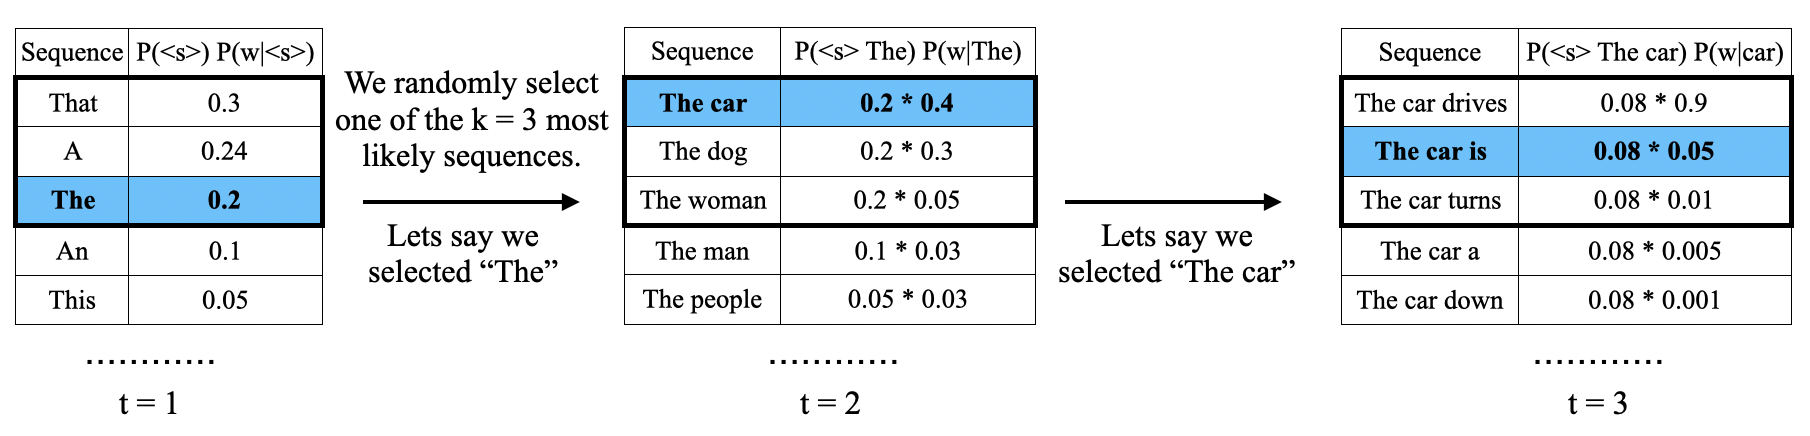
\includegraphics[width=0.92\textwidth]{images/top_k_sampling.png}
    \caption{Example of top-k random sampling. At each timestep t, the model generates the probability of the possible next word. Then, we randomly sample from the $k$ most likely candidates from this distribution. Here, we consider $k = 3$. \textbf{Bold} sequences represent the sampled candidate at each timestep.}
    \label{fig:top_k}
\end{figure}
    
    Once again, consider the bigram language model in Table \ref{tab:bigram_prob}.
    
    \begin{enumerate}
        \item (\textbf{1 pt}) Given the prefix string ``$\langle s\rangle\;I\;know$'', run the top-k sampling approach for the next 3 tokens.  Let $S$ be the set of output sequences that this approach could possibly generate at the end of 3 steps. What is the size of $S$? Assume $k = 2$ and $P(\langle s  \rangle\;I\;know) = 1$. You can just report the number.
        
        
        \item (\textbf{1 pt}) What is the sequence with maximum probability in $S$? Report the sequence and the probability of the sequence. 
        
        
        \item (\textbf{1 pt}) What is the sequence with  minimum probability in $S$? Report the sequence and the probability of the sequence.
        
        
    \end{enumerate}

    \item Let's say we are decoding a sentence of length $T$ using a language model with vocabulary size $V$. Report the time complexity in the big $O$ notation when the sentence is decoded using the following strategies:

    \begin{enumerate}
    \item (\textbf{1 pt}) Greedy search, where we store only the topmost sequence at each time step. 
    

    
    \item (\textbf{1 pt}) Beam search of width $k$, where we store the top-$k$ sequences at each time step: 


    
    \item (\textbf{1 pt}) Exhaustive search, where we store all the sequences at each time step: 
    
    
    \end{enumerate}

\end{enumerate}

\end{document}
